% Chapter Template

\chapter{Classical numerical results} % Main chapter title

\label{Chapter3} % Change X to a consecutive number; for referencing this chapter elsewhere, use \ref{ChapterX}


%----------------------------------------------------------------------------------------
%	SECTION 1
%----------------------------------------------------------------------------------------

In this section will we look at the two classical valuaing algorithms in computational finance the Binomial model and the Least Square Monte Carlo (LSM) approach. The models will both serve as reference for the Machine Learning model and provides insight into valuation of American options.

%-----------------------------------
%	SUBSECTION 1
%-----------------------------------

\section{Binomial Pricing model}
The Binomial model provides an intuitive and easy implementable model for valuing American and European options. The Binomial model comes handy, when no analytical model exists for American options. The Binomial model also has its limitations, because it is not suited for valuing path dependent options or options with several underlying factors. The key difference on the Binomial model and the other numerical procudures is that the Binomial model is build on a discrete framework. \\

The central concepts arbitrage and completeness from continuous time also work in the discrete time setup. The paper \parencite{binomial-Paper} which introduced the binomial model to option pricing came after the Black-Scholes model described in section \ref{Chapter2} \parencite{B-S-Paper}. The main reason for developing a model in discrete time, is that the the discrete time approach gives a simplified model in terms of the mathematics and highlights the essential concepts in option pricing theory. You can argue that the simpler mathematics in this model makes the binomial model more instructive and clear. Besides being easier to understand for non-mathematician it works nicely with other options than the European options like American options.\\

Eventhough we assume the stock price moves at discrete time instead in continuous time. It can actually be shown for a European Option that if the number of timesteps in the tree aproaches infinity, then the binomial model will converge to the continuous time closed form solution for a European option \parencite{binomial-Paper} \parencite{Hull}. Hence the binomial pricing model will be equivalent with the continuos time analytical pricing model derived by Fischer Black and Myron Scholes in the limit for european options \parencite{binomial-Paper}.\\

To value a american put option, we lay out all the possible path of the stock, based on the $S_0,\sigma$ and $T$. We need to specify the number of timesteps ($\Delta t = \frac{T}{N} \ where \ N=No. \ of  \ steps$) for the tree, where for each step, we add another possible value for the stock. We only add 1 more possibility for each timestep because the tree recombines. The precision for the algorithme increases with the number of steps and the option value stabilizes (see Figure \ref{fig:binConv}). For valuing an american put option, we value the exercise value at maturity (time T) for all possible outcomes for the stock. Then we work backward in the tree by comparing intrinsic value with the conditional expectation, where we choose the maximum of these two \parencite{Hull}. 
 
\begin{figure}[th]
\centering
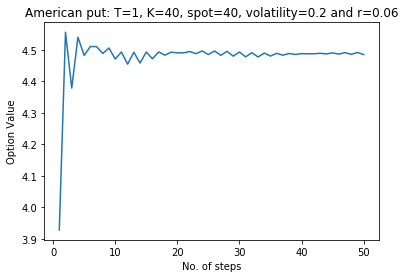
\includegraphics{Figures/binConv.png}
\decoRule
\caption[Convergence of Binomial model]{}
\label{fig:binConv}
\end{figure}


%-----------------------------------
%	SUBSECTION 2
%-----------------------------------


\subsection{Mathematics in Binomial valuation model}
The mathematics behind the binomial model is simpel and we will in this section provide the basic mathematics. First we need to construct the tree, then afterwards work backwards in the tree for valuation. For each time step ($\Delta t$), we assume the stock (S) can move up (u) or down (d). In order to avoid arbitrage we find the risk neutral measure q for the binomial tree, where q is the probability for the stock moves up. The risk neutral measure q is chosen s.t. the expected return is the risk-free rate r.

\begin{theorem}\label{RNVF-Discrete}
\textbf{Risk-neutral valuation formula in discrete time. }
Assume there exists a risk free asset. Then the market is arbitage free if and only if there exists a risk neutral measure $Q \sim P$ s.t.
\begin{align}
s= \exp(- r \Delta t) \cdot E^Q[S(t+\Delta t)|S(t)=s] 
\end{align}
Where $\Delta t$ is a single timestep.
\end{theorem}
From the above theorem, we can calculate the risk neutral mesure as:\\
$$q=\frac{e^{\Delta t}-d}{u-d}$$

The d and u is chosen s.t. they match volatility. So we choose:
$$u= \exp(\sigma \sqrt{\Delta t}) \quad d= \exp(-\sigma \sqrt{\Delta t})$$
Now we have determined the three parameters needed for constructing a binomial tree \parencite{binomial-Paper} \parencite{Hull} \parencite{finKont}.\\

We want to value an American put option, hence we need to work backward in the tree and comparing in each node the intrinsic value with the conditional expection (see theorem \ref{RNVF-Discrete}) by:
\begin{equation}
max\{ K-S(t), \exp(- r \Delta t) \cdot E^Q[P(t+\Delta t,T)|P(t,T)=p] \}
\end{equation}
The comparision will be applied for every node in each timestep $\Delta t$  and all the way back in time to the initialization date. By this precedure we get present value of the American option at initialization.



%----------------------------------------------------------------------------------------
%	SECTION 2
%----------------------------------------------------------------------------------------

\section{Least Square Monte Carlo Method}
The other classical result in this section is of an different nature, because it is based on simulation and linear regresion. In our setting we regress the expected payoff by continuation of the contract and compare it to the intrinsic value. The dependent variable in the regression is the expected value of continuation and the independent variables is a set of othogonal basis functions in $L^2(\Omega, \mathcal{F}, Q)$ of the simulated paths. Typical choices for basis functions could be weighted Laguerre -, Hermit -, and Jacob polynomials. This kind of regression is a nonlinear expansion of the linear model. In order to create data, we will simulate paths according to the underlying risky asset. 

\subsection{LSM method for an American put}           
We want to valuate an American put option with a stock as underlying asset. We take the same assumptions as in Chapter \ref{Chapter2} (see assumption \ref{BS-Assumption}) except the option is an American option. Hence in order to simulate the paths of the stock, we simulate from an GBM: $dS(t)=rSdt + \sigma S dW_t$ where $\sigma$ and r is constant (see solution to SDE equation \ref{GBM}). We simulate 100.000 paths for the stock. Like in the binomial model, we work backward to decide the optimal stopping time. The computer is discrete, hence we simulate the stock path as an Bermuda option, where we have 50 timesteps per year. I.e. we approximate the American option with a Bermudan option on same underlying. \\

At maturity the cashflow from the option is the same as for an European put option, hence the cashflow from each path is $C(\omega,T;T, T)=max(K-S_T,0)$. We use the notation $C(\omega, s; t, T)$ denote the path of cash flows generated by the option condition on the option not being exercised before t and the option holder follw the optimal stopping strategy for all s, $t<s\leq T$.
(inspired by \parencite{lsm} p. 121). The continuation value is given by:
\begin{equation}\label{continuation-value}
\begin{split}
F(\omega; t_k)=E^Q[\sum_{j=k+1}^K \exp(-\int_{t_k}^{t_j} r(\omega,s) ds)C(\omega,t_j; t_k, T)|\mathcal{F}_{t_k}]
\end{split}
\end{equation}
where $r(\omega,t)$ is risk free interest rate, and the $\mathcal{F}_{t_k}$ is the filtration at time $t_k$.\\

The optimal stopping strategy is then by comparing this continuation value with the intrinsic value at each time step. By working backward in time until the initialization of the option, we have specified the optimal stopping times and the cashflows associated with exercising at the optimal stopping times. To estimate the condition expection in equation \ref{continuation-value}, we regres with the basis functions taking on the underlying asset for the option being the independent variable:
$$F(\omega;t_{K-1})= \sum_{j=0}^\infty a_j L_j(X)$$
where a is the coefficients for the regression, L is the basis function, where the argument is the underlying asset $X$ \parencite{lsm}.

\subsection{Numerical results}
By the above two algorithms for valuation, we choose to vary spot, volatility and maturity for pricing an American put option with K=40 and r=0.06. This table will serve as reference for the machine learning algorithm in chapter (!TODO chapter for machine learning). For the binomial tree we use 100 timesteps, which gives stable results (compare to figure \ref{fig:binConv}) and for the lsm we use $10^5$ paths with 50 timesteps per year. The European option is valued by using BS closed form solution for a call option (see proposition \ref{BS-price-EuroCall}) and Put-call parity (see proposion \ref{Put-call-parity}).
\begin{table}[th]
\caption{Valuation of American put option with K=40 and r=0.06.}
\label{tab:treatments}
\centering
\begin{tabular}{l l l l l l l }
\toprule
\textbf{Spot} & \textbf{$\sigma$} & \textbf{T} & \textbf{Closed form European} & \textbf{Binomial Tree} & \textbf{LSM} & \textbf{abs. diff.} \\
\midrule
36 & 0.2 & 1 & 3.844 & 4.488 & 4.478 & 0.010\\
36 & 0.2 & 2 & 3.763 & 4.846 & 4.828 & 0.018\\
36 & 0.4 & 1 & 6.711 & 7.119 & 7.092 & 0.027\\
36 & 0.4 & 2 & 7.700 & 8.508 & 8.500 & 0.008\\
38 & 0.2 & 1 & 2.852 & 3.260 & 3.245 & 0.015\\
38 & 0.2 & 2 & 2.991 & 3.748 & 3.735 & 0.013\\
38 & 0.4 & 1 & 5.834 & 6.165 & 6.144 & 0.021\\
38 & 0.4 & 2 & 6.979 & 7.689 & 7.665 & 0.024\\
40 & 0.2 & 1 & 2.066 & 2.316 & 2.313 & 0.003\\
40 & 0.2 & 2 & 2.356 & 2.885 & 2.881 & 0.004\\
40 & 0.4 & 1 & 5.060 & 5.310 & 5.326 & 0.016\\
40 & 0.4 & 2 & 6.326 & 6.914 & 6.908 & 0.006\\
42 & 0.2 & 1 & 1.465 & 1.622 & 1.622 & 0.000\\
42 & 0.2 & 2 & 1.841 & 2.217 & 2.212 & 0.005\\
42 & 0.4 & 1 & 4.379 & 4.602 & 4.596 & 0.006\\
42 & 0.4 & 2 & 5.736 & 6.264 & 6.243 & 0.021\\
44 & 0.2 & 1 & 1.017 & 1.117 & 1.113 & 0.004\\
44 & 0.2 & 2 & 1.429 & 1.697 & 1.688 & 0.009\\
44 & 0.4 & 1 & 3.783 & 3.956 & 3.962 & 0.006\\
44 & 0.4 & 2 & 5.202 & 5.656 & 5.649 & 0.007\\
\bottomrule\\
\end{tabular}
\end{table}
We see the maximum difference between the two algorithms is 0.027 at S=38, $\sigma=0.4$ and T=2. The other obvious fact is that the european put has a lower value than its American counterpart, because the continuous exercise feature adds additional value to the put option. 
